\documentclass[a4paper,11pt,uplatex]{jsbook}
%\usepackage{fancyhdr}
\setlength{\footskip}{16pt}
\usepackage{amsmath}
\usepackage[dvipdfmx]{graphicx}
\usepackage[dvipdfmx]{color}
%\usepackage{pagecolor}[white]
\usepackage{amsmath,amssymb}
%\usepackage[top=3cm, bottom=3cm, left=3cm, right=3cm]{geometry}
\usepackage{braket}
\usepackage{bm}
\numberwithin{equation}{section}
\usepackage{mathrsfs}
\usepackage{siunitx}
\usepackage{physics}
\usepackage[dvipdfmx]{graphicx}
\usepackage[compat=1.1.0]{tikz-feynhand}
\usepackage{caption}
\usepackage{subcaption}
%\usepackage{cleveref}
\usepackage{float}
\usepackage{multicol}
\setlength{\columnsep}{15mm}
%\usepackage[style=phys,articletitle=false,biblabel=brackets,chaptertitle=false,pageranges=false]{biblatex}
%\usepackage[style=phys]{biblatex}
\usepackage[dvipdfmx]{hyperref}
\usepackage{url}
\usepackage{pxjahyper}
\usepackage{bookmark}
%\usepackage[backref]{hyperref}
\setcounter{tocdepth}{3}
\setlength{\parindent}{2em}
\def\vector#1{\mbox{\boldmath $#1$}}
\def\slash#1{\not\!#1}
\def\slashb#1{\not\!\!#1}
\def\delsla{\not\!\partial}
%\usepackage[dvipdfmx]{xcolor}


\hypersetup{
 setpagesize=false,
 bookmarksnumbered=true,%
 bookmarksopen=true,%
 colorlinks=true,%
 linkcolor=black,
 citecolor=red,
 urlcolor=black,
}
%backreferenceのカスタマイズ. "Back to p.3"のように表示する.
%\renewcommand*{\backref}[1]{(p.#1へ戻る)}
%\newcommand{\backtoc}{\hyperlink{toc}{[目次へ]}}
\newcommand{\backtoc}{\texorpdfstring{\protect\hyperlink{toc}{\hspace{5pt} \scriptsize [目次へ]}}{}}
\newcommand{\mychapter}[1]{\chapter[#1]{#1\backtoc}}
\newcommand{\mysection}[1]{\section[#1]{#1\backtoc}}
\newcommand{\mysubsection}[1]{\subsection[#1]{#1\backtoc}}

% 数式
%\usepackage{amsmath,amsfonts}
%\usepackage{bm}
%\usepackage{physics}
% 画像
%\usepackage[dvipdfmx]{graphicx}
%\usepackage[dvipdfmx,colorlinks=true,linkcolor=blue]{hyperref}
%\usepackage{pxjahyper}

\begin{document}

\chapter{結果}
\section{結果}
\subsection{画像処理}
各ピクセルの同一位置での4枚の画像の平均値と標準偏差の関係を示す。
周囲のピクセルの平均値に対する超過の値は以下のような分布となる。
\subsection{波長較正}
水銀灯を用いて波長較正を行った結果の一例を示す。
ピーク位置決定精度は0.1 nm程度である。

\subsection{単独アンジュレータ}
下流側のアンジュレータのみを用いて取得したデータの解析結果を示す。
このデータを用いてパラメータの較正をおこなった。
\subsubsection{波長依存性}
波長依存性があり長波長側の光量が大きい傾向がある。
この傾向は線形の依存性が仮定できる。\\
\subsubsection{位置依存性}
アンジュレータの位置に対する依存性があり、アンジュレータが下流に移動するにつれて3つの傾向が見られる。
\begin{itemize}
  \item 回折パターンの振幅が上昇する
  \item 回折パターンの形状が変化する
  \item 回折パターンの振幅が周期的に小さく変動する
\end{itemize}
振幅の上昇と周期的な変動は放射角に対して一様ではない。特にピーク位置を抽出して振幅の変化をみると、
ピークごとに異なる上昇率が見られる。これはアンジュレータ位置に対して回折パターンの形状も変化することが影響していると推定できる。
一方で回折パターンの振幅はどのピクセルにおいてもほぼ一定であり、その振幅は電子ビームエネルギー210 MeVの振幅と対応している。
偏極電磁石による一定位相の放射との干渉が見えていると考えることができる。
実際に一定位相の偏極電磁石放射を仮定してシミュレーションした結果によれば、振幅の傾向は一致する。\\
\subsubsection{放射光および光学系パラメータ}
回折パターンの形状を決定するパラメータはアンジュレータ - スリット間距離、スリット - カメラ間距離、スリット幅の3つである。
これに加えて放射光関数の情報も形状を決定する。放射光関数の形状は理論式を仮定し、z(U2-slit)、z(slit-cam)、w(slit)の3つのパラメータの最適値を決定する。\\
アンジュレータと光学系の距離に依存して光量が変化する。立体角を考えるとこの光量はスリットからの距離rに対して$\frac{1}{r^2}$に比例すると考えられる。
また距離によって振幅が周期的に変動する効果は、偏極電磁石による放射だと考えることができる。
このような仮定に基づいて単独アンジュレータのデータをフィットした。\\
またパラメータを固定した時の適合度の比較の結果を示す。
これらの結果からパラメータの値を??と決定した。
またパラメータの決定精度は??である。
\section{電子ビームエネルギーの測定結果}
\subsubsection{}
2台のアンジュレータの放射光による干渉パターンの解析結果を示す。
下流アンジュレータの位置に対して図が示すように干渉パターンの中心の振幅が周期的に変化する。
回折パターンを距離とy軸の関数としてフィットした結果の例を示す。
位置の変化に対しても回折パターンの形状をフィットできていることがわかる。
\subsubsection{パラメータの統計誤差}
ブートストラップ法によってフィッティングパラメータの誤差を見積もった。
またパラメータ同士の相関係数を計算すると、??が となった。
それ以外の相関係数は全て0.1以下である。
特に$\gamma$パラメータの統計誤差は表の通りとなった。
このことから電子ビームエネルギーは??の精度で決定できることがわかる。
\subsection{系統誤差}
\subsubsection{波長依存性}
異なる波長でエネルギーを決定し、その結果から波長依存性による系統誤差を見積もった。
\subsubsection{距離依存性}
下流側アンジュレータの位置を4つの区間に分割し、各区間でエネルギーを決定した。
これによりフィット関数が持つ位置依存性による系統誤差を見積もることができる。

\subsubsection{エネルギー依存性}
180,195,210 MeVの3つのエネルギーの結果を表に示す。













\clearpage

\begin{figure}[tb]
  \centering
  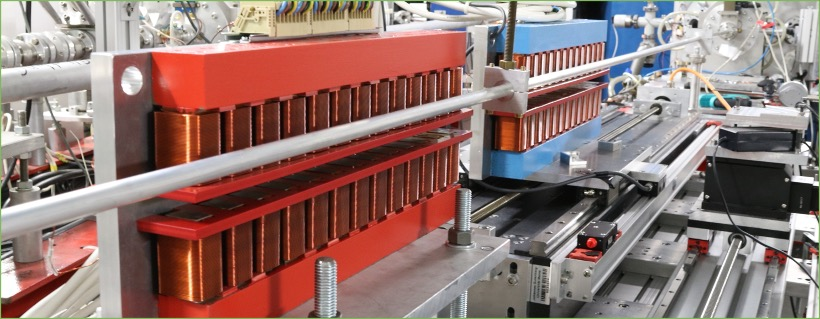
\includegraphics[width=0.8\linewidth]{image/1-1.jpg}\\
  \caption{サンプルの図}
  \label{sample_image}
\end{figure}

\begin{itemize}
  \item a
\end{itemize}
\begin{enumerate}
  \item b
\end{enumerate}

\begin{align}
\frac{1}{2} = \qty(\frac{1}{3}) + \qty{1}\Sigma
\end{align}
\end{document}